\chapter{Phân tích Dữ liệu Thị trường Chứng khoán Việt Nam}
\vspace{-2.5em}

Ngoài dữ liệu từ diễn đàn FireAnt, thị trường chứng khoán Việt Nam là đối tượng phân tích tiếp theo của ta. Thị trường cũng cung cấp lượng data ``màu mỡ'' để ta có thể khai thác, và củng cố giả thuyết.

\section{Phân tích các mã cổ phiếu theo ngành}

\subsection{Phân bổ giữa các ngành}
\begin{center} 
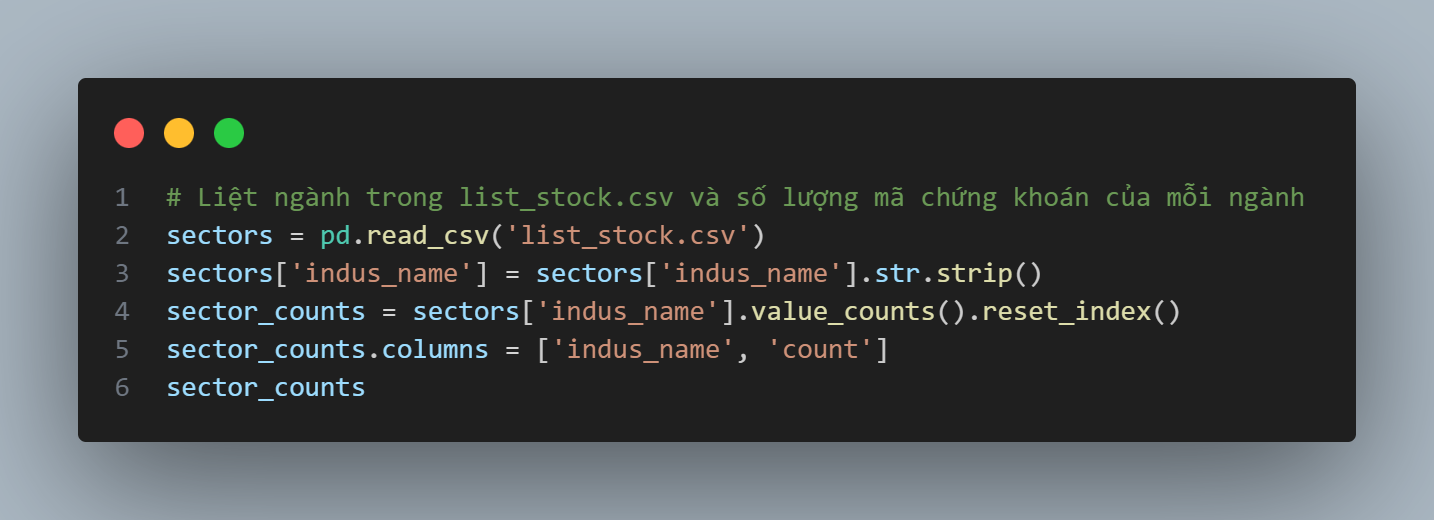
\includegraphics[width=0.7\linewidth]{images/code-2.20.png}
\end{center}

Ta sẽ bắt đầu bằng việc nhập file \texttt{list\_stock.csv}. Ta sẽ sử dụng dữ liệu về nhóm ngành của từng công ty niêm yết trong danh sách.
\vspace{-0.5em}
\begin{figure}[H]
    \centering
    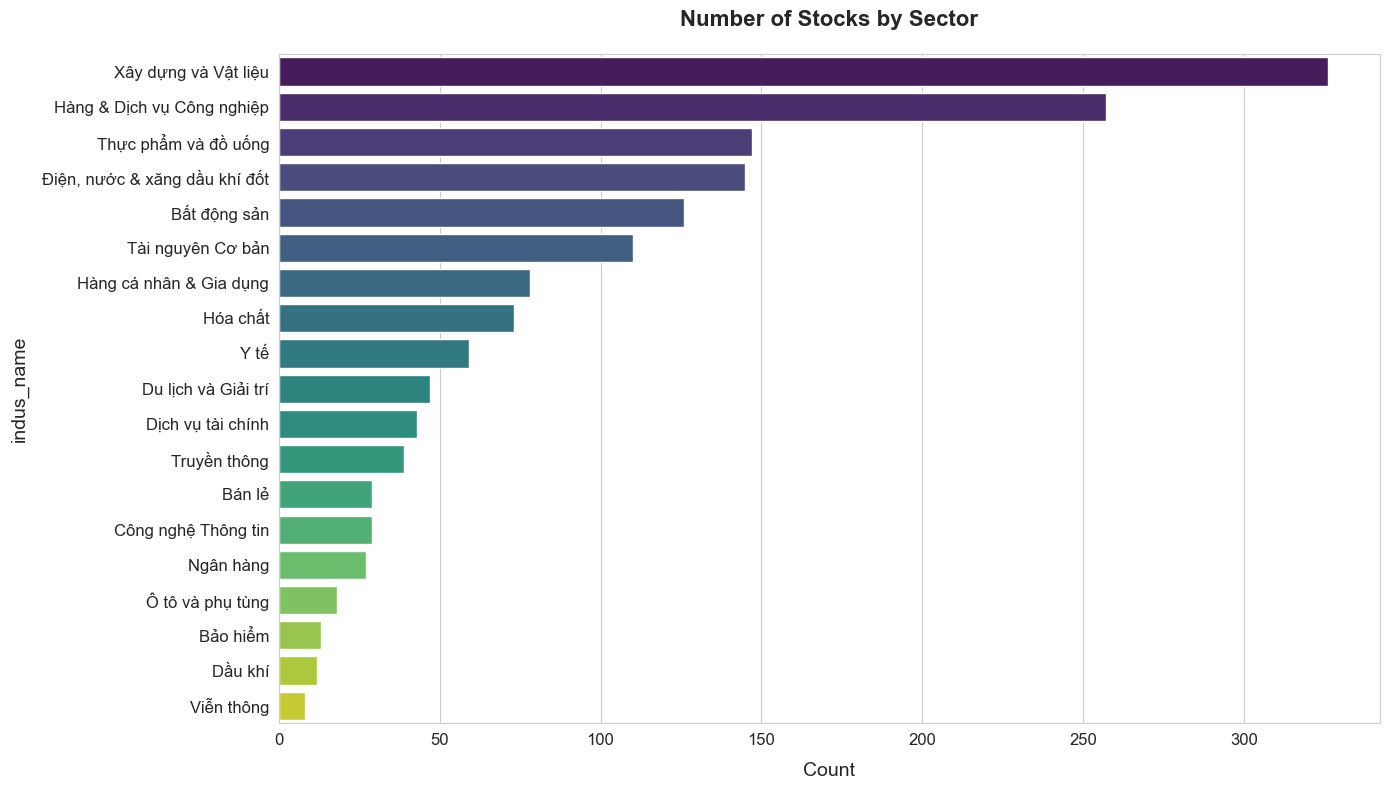
\includegraphics[width=1\linewidth]{images/plot-3.8-bar_chart.png}
    \vspace{-2em}
    \caption{Số lượng mã cổ phiếu trong ngành}
    \label{fig:3.1}
\end{figure}

\textbf{Nhận xét:}
\begin{itemize}
    \item Ngành \textbf{Xây dựng và Vật liệu} là ngành có số lượng cổ phiếu cao nhất, vượt trội so với các ngành khác. Sau đó là \textbf{Hàng Dịch vụ Công nghiệp}, có số lượng cổ phiếu gần tương đương với ngành dẫn đầu. Ngành \textbf{Thực phẩm và đồ uống} và \textbf{Điện, nước xăng dầu khí đốt} cũng có số lượng cổ phiếu đáng kể, nhưng thấp hơn so với hai ngành đầu tiên. Các ngành như \textbf{"Viễn thông", "Dầu khí",} và \textbf{"Bảo hiểm"} có số lượng cổ phiếu thấp nhất trong biểu đồ.
    \item Tóm lại, có sự chênh lệch rõ rệt giữa các ngành, và trong phân bổ ngành kinh tế Việt Nam. Một số ngành có số lượng cổ phiếu áp đảo trong khi nhiều ngành khác tương đối thấp.
\end{itemize}

\subsection{Vốn hóa thị trường, số cổ phiếu lưu hành}
Vốn hóa và số cổ phiếu lưu hành luôn là nhưng tiêu chí có sức ảnh hưởng lớn tới việc mua bán mã chứng khoán. Dưới đây là biểu đồ mô tả 2 giá trị quan trọng đó với từng ngành:

\begin{center}
    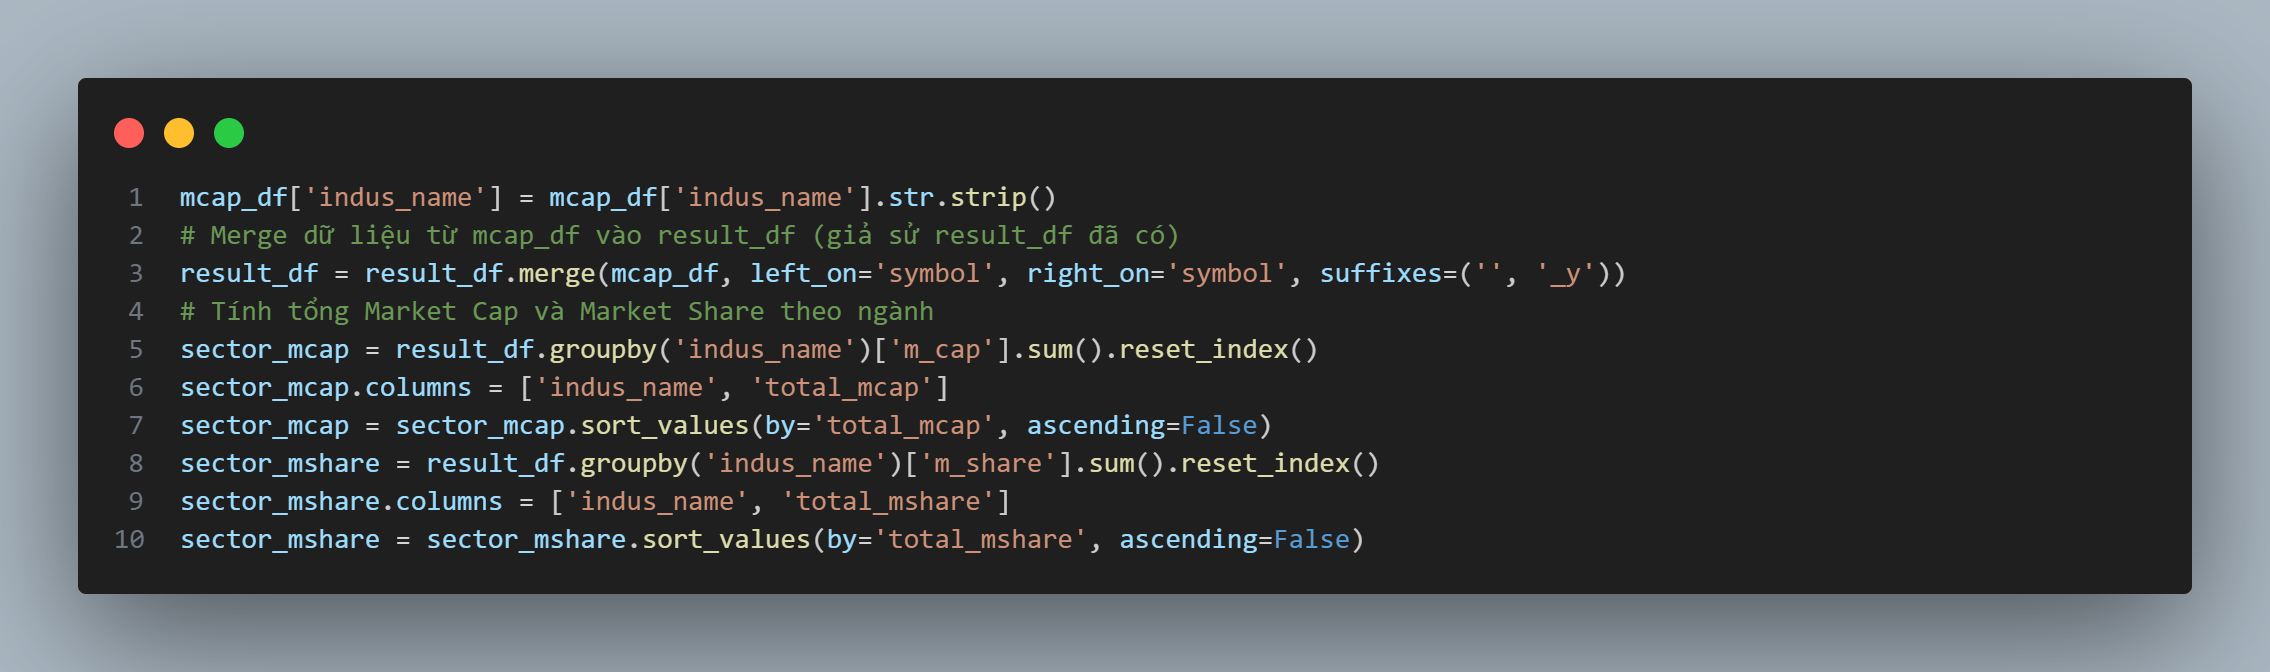
\includegraphics[width=1\linewidth]{images/code-3.19.png}
\end{center}

\begin{figure}[H]
    \centering
    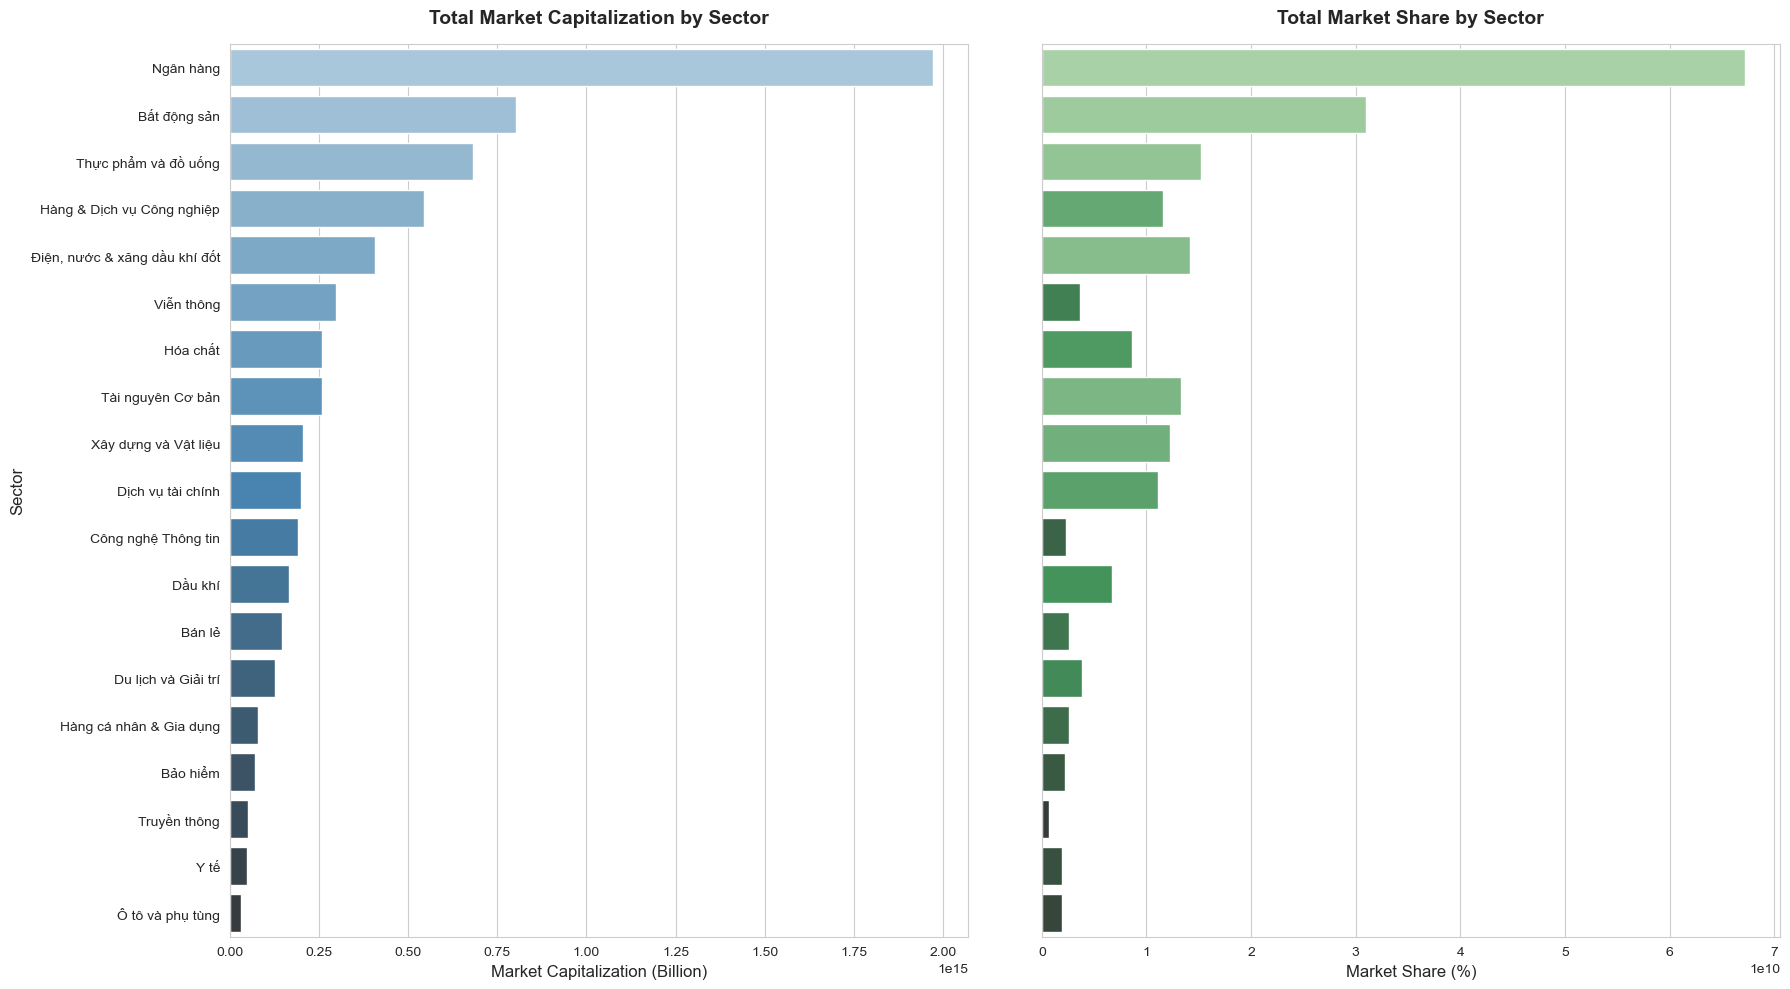
\includegraphics[width=1\linewidth]{images/plot-3.9-column_chart_merged.png}
    \caption{Vốn hóa thị trường và Số cổ phiếu lưu hành}
    \label{fig:3.2}
\end{figure}

\textbf{Nhận xét:}
\begin{itemize}
    \item \textbf{Ngân hàng} là ngành có lượng vốn và cổ phiếu lưu hành nhiều nhất dẫu cho số mã chứng khoàn của ngành này khá khiêm tốn so với tất cả các ngành khác. Theo sau \textbf{Ngân hàng} là các ngành như \textbf{Bất động sản}, \textbf{Thực phẩm và đồ uống}, ...
    \item Có thể thấy rằng không phải vốn hóa cao cũng đồng nghĩa với số cổ phiếu lưu hành cao.
\end{itemize}

\newpage
\subsection{Quan điểm người dùng}
Tương tự, ta lấy cột tên ngành từ \texttt{list\_stock.csv} kết hợp để lập biểu đồ với số lượng bài viết thể hiện quan điểm Tích cực hoặc Tiêu cực.

\begin{center} 
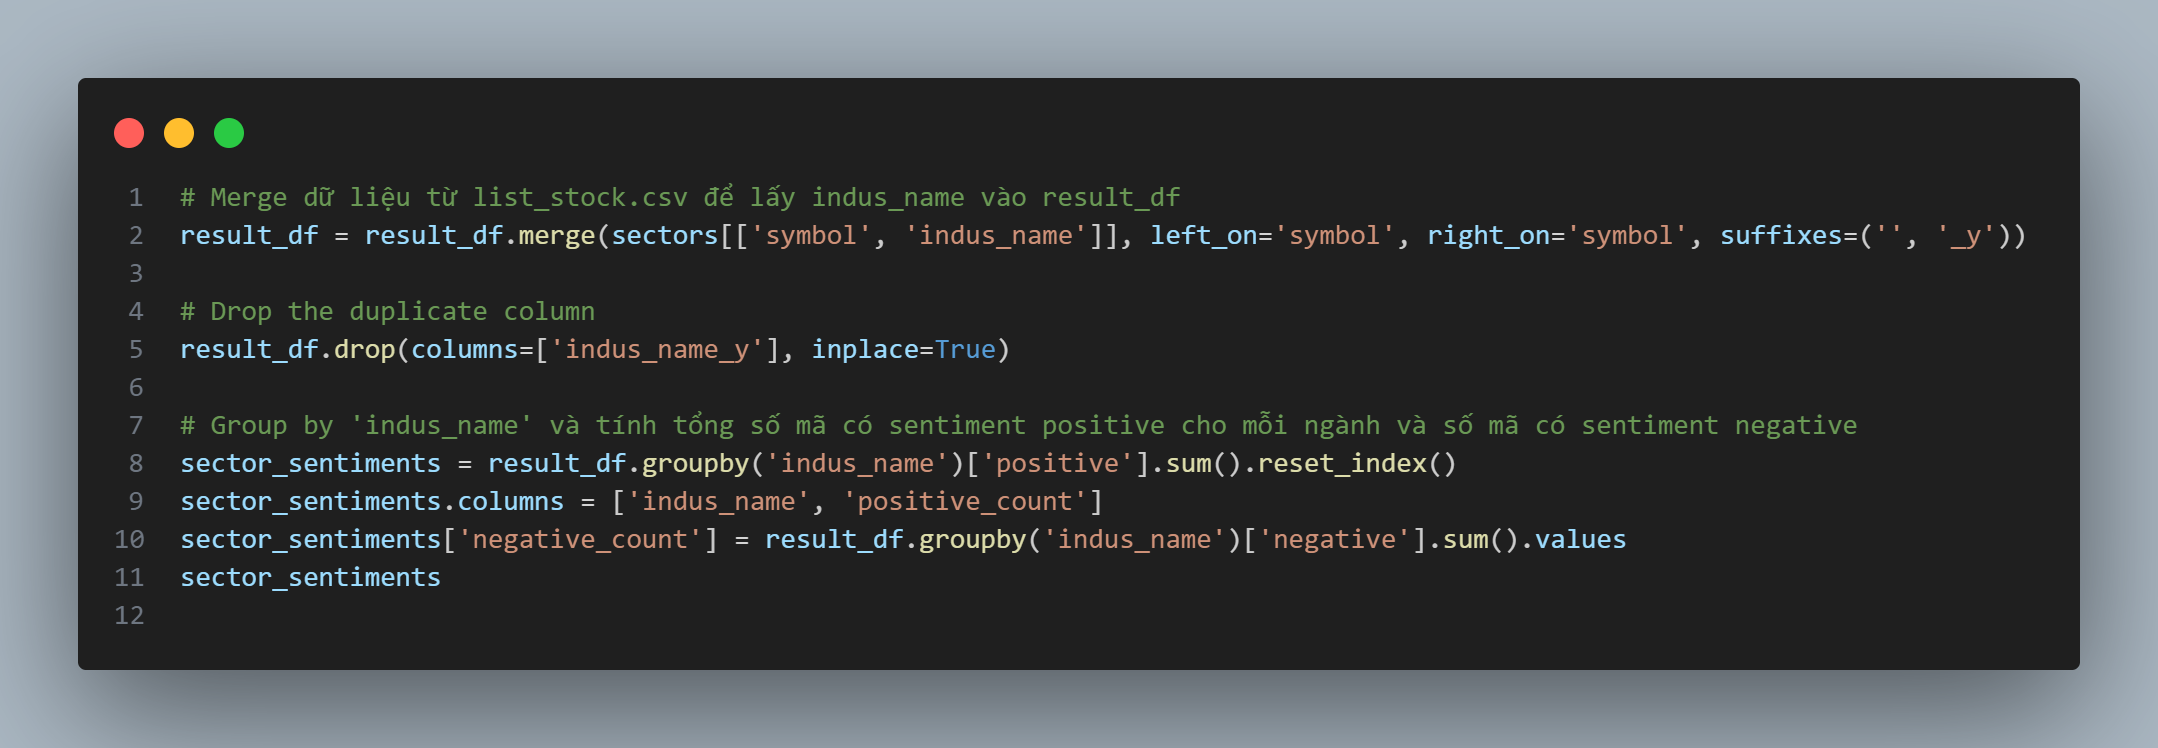
\includegraphics[width=1\linewidth]{images/code-2.2-sentiments.png}
\end{center}

\begin{figure}[H]
    \centering
    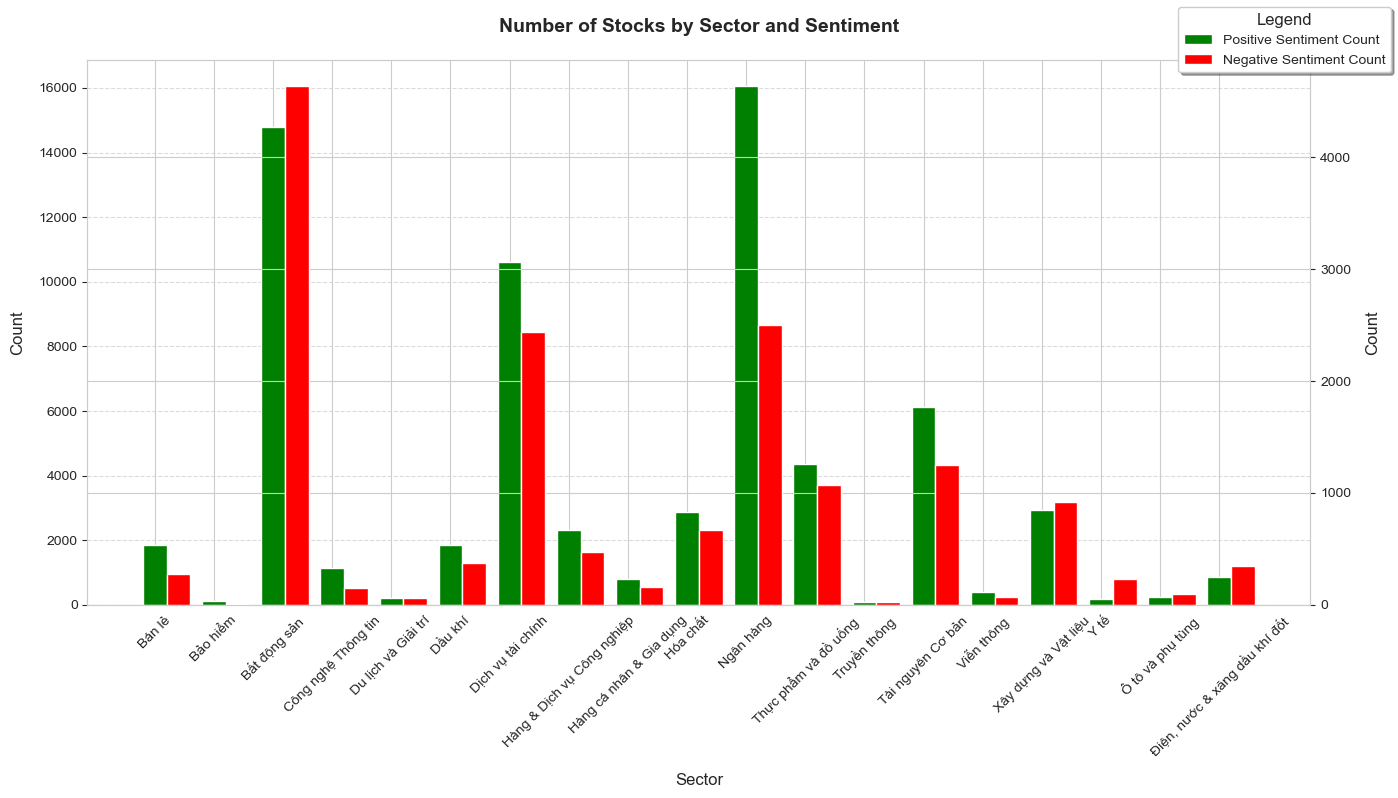
\includegraphics[width=1\linewidth]{images/plot-2.18-column_chart.png}
    \caption{Biểu đồ phản ánh ngành và Quan điểm của người dùng}
    \label{fig:3.3}
\end{figure}
\textbf{Nhận xét:}

\begin{itemize}
    \item Các ngành có số lượng bài viết nhiều là \textbf{Bất động sản, Dịch vụ tài chính (Chứng khoán), Ngân hàng, Tài nguyên, Xây dựng và Vật liệu}.
    \item Đa phần các ngành đều có lượng bài viết Tích cực cao hơn Tiêu cực, nhưng có một vài ngoại lệ như ngành \textbf{Bất động sản}, do đa số các mã trong ngành này chịu ảnh hưởng xấu trong khoảng thời gian lấy dữ liệu.
    \item Ngành \textbf{Ngân hàng} có chỉ số Tích cực gấp đôi, do đây là ngành được hưởng lợi và các mã trong ngành đều tăng trưởng rất tốt trong khoảng thời gian lấy dữ liệu.
\end{itemize}

\section{Phân tích Tương quan}
\subsection{Tương quan trong Thị trường Nội địa}

Trên thị trường chứng khoán Việt Nam, có 3 chỉ số thị trường lớn là VNINDEX, VN30 và HNXINDEX. Dưới đây là khối lượng giao dịch của 3 mã theo ngày.

\begin{center}
    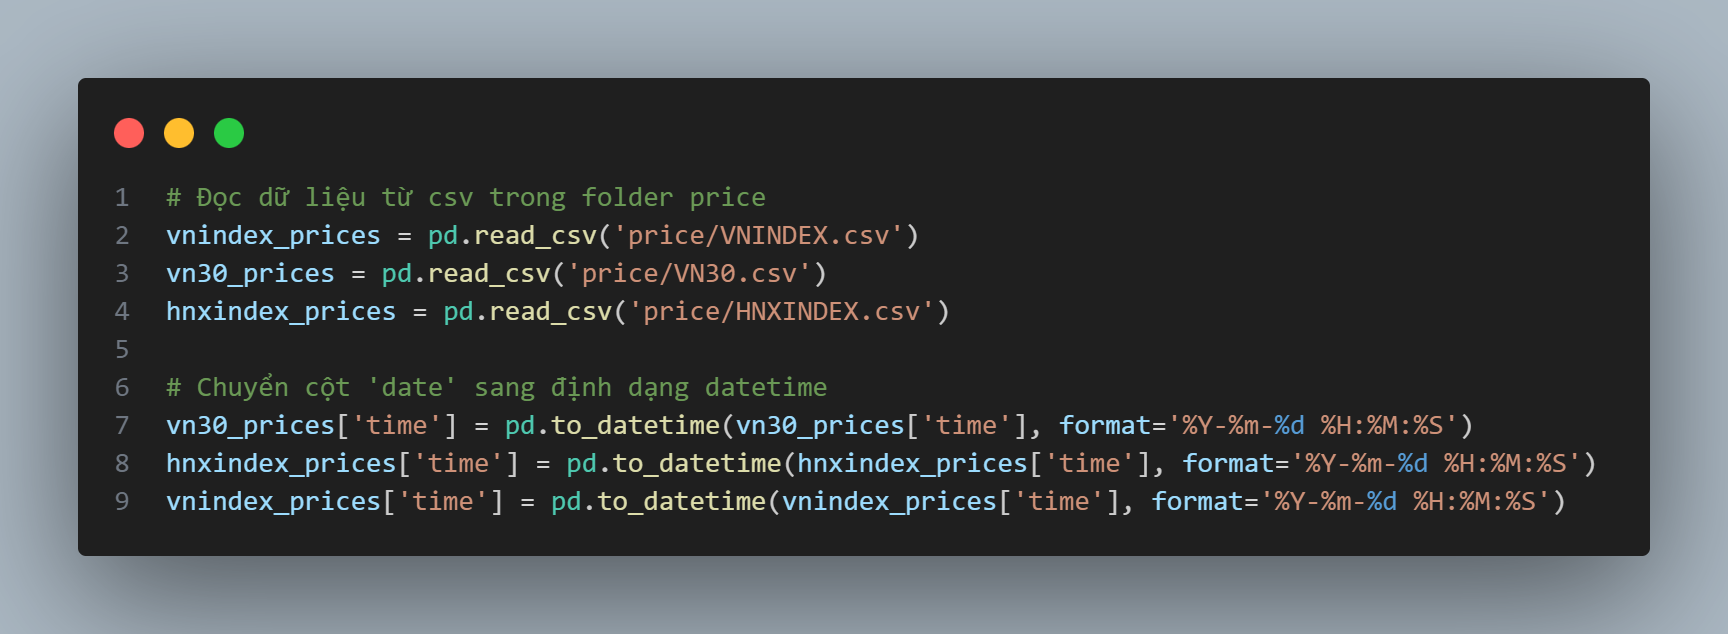
\includegraphics[width=0.9\linewidth]{images/code-2.21.png}
\end{center}
\begin{figure}[H]
    \centering
    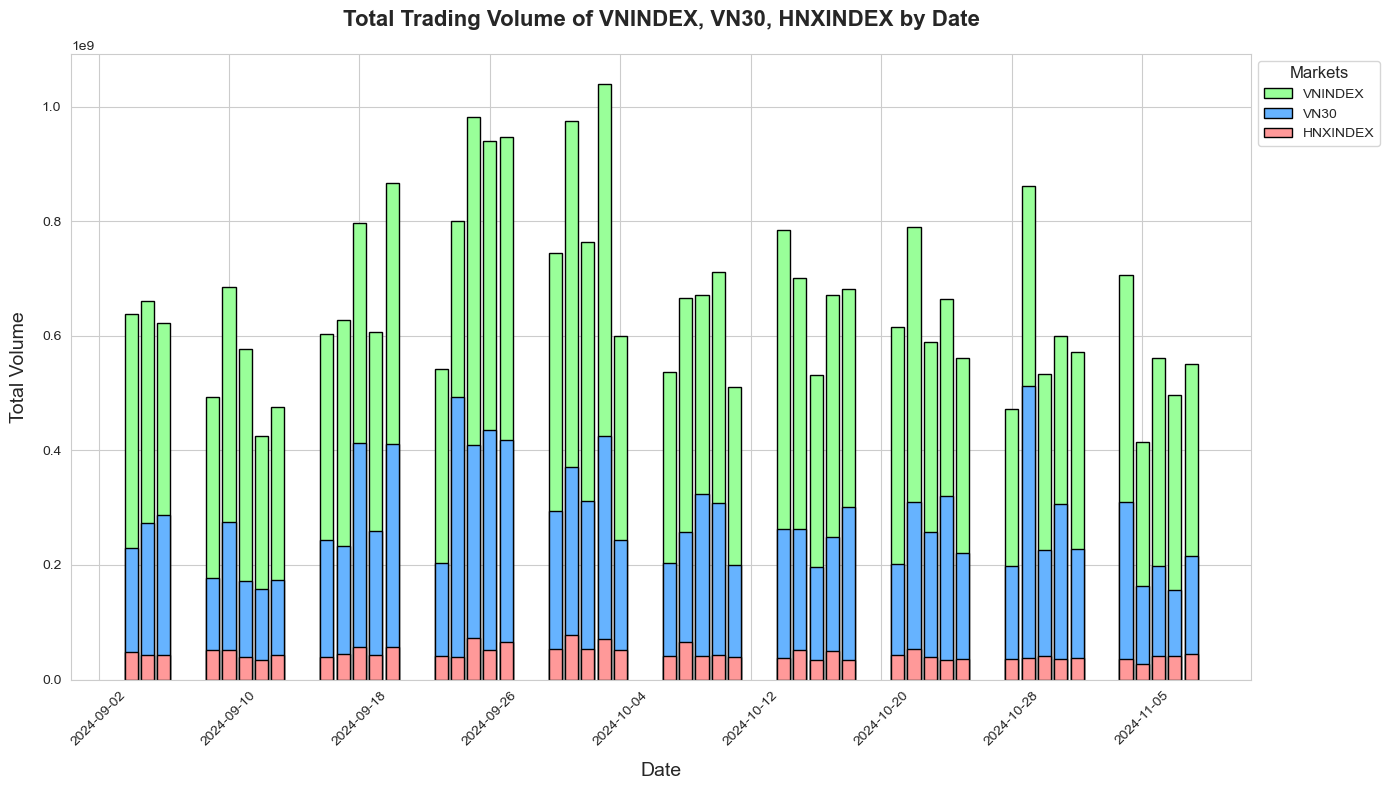
\includegraphics[width=1\linewidth]{images/plot-2.6-column_chart.png}
    \caption{Khối lượng giao dịch của VN30, VNINDEX, HNXINDEX}
    \label{fig:3.4}
\end{figure}
\textbf{Nhận xét:}
\begin{itemize}
    \item Có xảy ra nhiều biến đổi mạnh, diễn ra vào cuối tháng 9 đầu tháng 10, khi chỉ số điểm VNINDEX giảm từ 1300 xuống 1265.
    \item Nhìn chung khối lượng của cả 3 chỉ số thị trường không có sự biến đổi quá rõ rệt, do có sự liên quan tới nhau và cùng chịu ảnh hưởng ở chung một nền kinh tế. Có thể thấy khá rõ sự đồng pha của các chỉ số thị trường chứng khoán Việt Nam.
\end{itemize}

\newpage
\subsection{Tương quan với Thị trường Nước ngoài}
Có thể thấy rằng nhịp đập của thị trường chứng khoán Việt Nam là một bản giao hưởng hài hòa, ma trận tương quan dưới đây sẽ vừa thể hiện rõ điều đó, cũng như là bổ sung thêm nhưng thông tin quan trọng về mối tương quan với thị trường ngoài nước. Ta sẽ sử dụng dữ liệu từ \texttt{investing.com}, chúng là phần dữ liệu được cào thêm:
\begin{figure}[H]
    \centering
    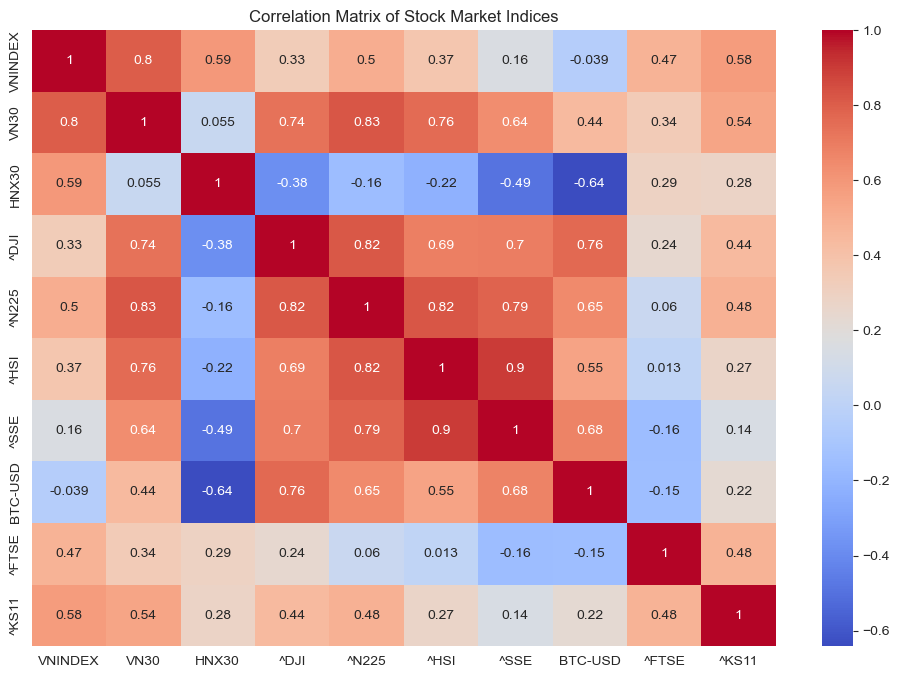
\includegraphics[width=1\linewidth]{images/plot-2.9-heatmap.png}
    \vspace{-1em}
    \caption{Ma trận tương quan giữa mã thị trường trong nước và quốc tế}
    \label{fig:3.5}
\end{figure}

\textbf{Nhận xét:}

\begin{itemize}
    \item VN30 và N225 (0.83): Mối tương quan cao giữa VN30 và Nikkei 225 cho thấy sự liên kết của thị trường Việt Nam với thị trường Nhật Bản.
    \item VN30 và DJI (0.74): Chỉ số VN30 có mối tương quan mạnh với Dow Jones, cho thấy sự ảnh hưởng của thị trường Mỹ đến thị trường châu Á. 
    \item VN30 và HSI (0.76): Thị trường Việt Nam có mối liên hệ khá mạnh với Hang Seng (Hồng Kông).
    \item VN30 và SSE (0.64): VN30 cũng có sự gắn kết với thị trường Trung Quốc.
    \item VNINDEX và VN30 (0.8): Chỉ số chung của Việt Nam có mối tương quan chặt chẽ với chỉ số nhóm vốn hóa lớn (VN30), điều này dễ hiểu do VN30 chiếm tỷ trọng cao trong VNINDEX.
    \item HNX30 và BTC (-0.64): Có sự đối lập giữa hiệu suất của HNX30 và tiền điện tử (Bitcoin).
    \item HNX30 và DJI (-0.38): HNX30 cũng có mối tương quan âm yếu với chỉ số Dow Jones, cho thấy ít liên hệ giữa sàn chứng khoán Hà Nội và thị trường Mỹ.
    \item Nhìn chung, các thị trường trong khu vực Châu Á (VN30, HSI, N225, SSE, KS11) có sự đồng pha mạnh, cho thấy sự ảnh hưởng qua lại trong khu vực. Nhưng HNX30 lại tương đối khác biệt so với các chỉ số khác.
 
\end{itemize}